    \UseRawInputEncoding
    \documentclass[12pt,a4paper]{article}
    \usepackage[utf8]{inputenc}
    \usepackage[portuguese]{babel}
    \usepackage{geometry}
    \geometry{top=3cm, bottom=2cm, left=3cm, right=2cm}
    \usepackage{graphicx}
    \usepackage{listings}
    \usepackage{xcolor}
    \usepackage{hyperref}
    \usepackage{booktabs}
    \usepackage{amsmath}
    \usepackage[T1]{fontenc}
    \usepackage{pmboxdraw}
    \sloppy
    \usepackage{longtable}

    \definecolor{codegray}{rgb}{0.5,0.5,0.5}
    \definecolor{codeblue}{rgb}{0.13,0.13,1}
    \definecolor{codegreen}{rgb}{0,0.6,0}
    \definecolor{backcolour}{rgb}{0.96,0.96,0.98}

    \lstdefinestyle{mystyle}{
        backgroundcolor=\color{backcolour},
        commentstyle=\color{codegreen},
        keywordstyle=\color{codeblue},
        numberstyle=\tiny\color{codegray},
        stringstyle=\color{magenta},
        basicstyle=\ttfamily\small,
        breakatwhitespace=false,
        breaklines=true,
        captionpos=b,
        keepspaces=true,
        numbers=left,
        numbersep=5pt,
        showspaces=false,
        showstringspaces=false,
        showtabs=false,
        tabsize=2
    }
    \lstset{style=mystyle}

    \hypersetup{
        colorlinks=true,
        linkcolor=blue,
        filecolor=magenta,
        urlcolor=cyan,
    }

    \begin{document}

    \begin{titlepage}
    \centering

    \vspace*{2cm}

    {\large UNIVERSIDADE DO ESTADO DO RIO GRANDE DO NORTE}

    \vspace{4cm}

    {\Large \textbf{Ferramenta de Segurança da Informação}}

    \vspace{0.5cm}

    {\Large \textbf{Wazuh SIEM}}

    \vspace{3cm}

    {\large
    DISCIPLINA: MDI 0209 -- SEGURANÇA DE SISTEMAS (08052051)\\[0.3cm]
    DOCENTE: ISAAC DE LIMA OLIVEIRA FILHO
    }

    \vspace{2cm}

    {\large EQUIPE:}\\[0.3cm]
    {\large
    EDUARDO MARINHO DE PAIVA\\
    JOÃO VICTOR AMARAL DE SOUZA\\
    LUIZ HENRIQUE ALVES FERREIRA\\
    MARLOS EMANUEL DA SILVEIRA FONTES\\
    PAULO SÉRGIO SILVA DE MEDEIROS\\
    VINÍCIUS EDUARDO FREITAS DE SALES
    }

    \vfill

    {\large MOSSORÓ -- RN\\2026}

    \end{titlepage}

    \newpage

    \tableofcontents
    \newpage

    % ===========================================================================
    \section{Introdução}
    % ===========================================================================

    \subsection{Apresentação do Tema Escolhido}

    O tema deste trabalho é a implementação e demonstração de um Centro de Operações de Segurança (SOC) corporativo utilizando a plataforma \textbf{Wazuh 4.9} como SIEM (\textit{Security Information and Event Management}) open source. O Wazuh é uma solução líder de mercado que integra funcionalidades de HIDS (\textit{Host-based Intrusion Detection System}), monitoramento de integridade de arquivos (FIM), detecção de vulnerabilidades e resposta ativa a incidentes, tudo em uma plataforma unificada e gratuita.

    \subsection{Contextualização do Problema}

    O cenário de ameaças cibernéticas na atualidade é caracterizado por ataques cada vez mais sofisticados, frequentes e com impactos financeiros e reputacionais significativos. O custo médio de uma violação de dados ultrapassou US\$ 4 milhões em 2023, e o tempo médio para identificação de um ataque é de aproximadamente 207 dias. As organizações enfrentam desafios como:

    \begin{itemize}
        \item Volume massivo de logs e eventos gerados por diferentes sistemas
        \item Dificuldade em correlacionar eventos aparentemente isolados em um ataque coordenado
        \item Necessidade de atender requisitos regulatórios (LGPD, ISO 27001, NIST CSF)
        \item Falta de visibilidade centralizada sobre a postura de segurança
        \item Resposta lenta a incidentes devido à falta de automação
    \end{itemize}

    \subsection{Objetivo da Ferramenta dentro da Segurança da Informação}

    O Wazuh tem como objetivo centralizar a coleta, normalização, correlação e armazenamento de eventos de segurança de múltiplas fontes (servidores, aplicações, firewalls, bancos de dados) em uma única plataforma, permitindo:

    \begin{itemize}
        \item Detecção em tempo real de ameaças e anomalias
        \item Correlação avançada de eventos para identificar ataques coordenados
        \item Mapeamento automático para frameworks de compliance (NIST CSF, ISO 27001, LGPD)
        \item Resposta automatizada a incidentes (bloqueio de IP, isolamento de processos)
        \item Geração de relatórios e dashboards para tomada de decisão
    \end{itemize}

    \newpage
    % ===========================================================================
    \section{Visão Geral da Ferramenta}
    % ===========================================================================

    \subsection{O que é a Ferramenta}

    O Wazuh é uma plataforma de segurança open source (licença GPLv2) que combina funcionalidades de SIEM, XDR (\textit{Extended Detection and Response}) e monitoramento de segurança em uma solução unificada. É composto por quatro componentes principais:

    \begin{itemize}
        \item \textbf{Wazuh Agent:} Agente leve instalado nos endpoints para coleta de logs, monitoramento de arquivos, detecção de rootkits e varredura de vulnerabilidades
        \item \textbf{Wazuh Manager:} Servidor central responsável pela análise e correlação de eventos recebidos dos agentes
        \item \textbf{Wazuh Indexer:} Cluster OpenSearch para armazenamento e indexação de alertas e eventos
        \item \textbf{Wazuh Dashboard:} Interface web baseada em OpenSearch Dashboards para visualização, busca e análise de dados
    \end{itemize}

    \subsection{Principais Funcionalidades}

    \begin{itemize}
        \item \textbf{Correlação de Logs em Tempo Real:} Coleta, normalização e análise de logs de sistema, aplicação e rede com mais de 1.400 regras pré-definidas e suporte a regras customizadas em XML
        \item \textbf{Monitoramento de Integridade de Arquivos (FIM):} Detecta alterações em arquivos críticos em tempo real, incluindo criação, modificação, exclusão e alteração de permissões. Suporta monitoramento em tempo real (\textit{realtime}) e por varredura periódica (\textit{scheduled})
        \item \textbf{Detecção de Vulnerabilidades e Compliance:} Varredura automatizada de CVEs em pacotes instalados, mapeamento para frameworks regulatórios (NIST CSF, PCI DSS, HIPAA, ISO 27001, LGPD/GDPR) e verificação de configurações seguras (SCA - Security Configuration Assessment)
    \end{itemize}

    \subsection{Casos de Uso Mais Comuns}

    \begin{itemize}
        \item \textbf{Monitoramento de Servidores Corporativos:} Coleta centralizada de logs de servidores Linux e Windows, detecção de tentativas de invasão, análise de integridade de arquivos críticos e identificação de malwares/rootkits
        \item \textbf{SOC e Detecção de Ameaças:} Correlação de eventos de múltiplas fontes para identificar ataques coordenados, geração de alertas em tempo real com níveis de severidade, e resposta automatizada (bloqueio de IP, execução de scripts)
        \item \textbf{Auditoria de Compliance Regulatório:} Mapeamento automático de eventos de segurança para controles de frameworks como LGPD, ISO 27001 e NIST CSF, geração de relatórios de conformidade e scorecards de maturidade
    \end{itemize}

    \subsection{Vantagens e Limitações}

    \subsubsection{Vantagens}

    \begin{itemize}
        \item \textbf{Código Aberto e Gratuito:} Sem custos de licenciamento, mesmo para grandes volumes de dados. Comunidade ativa e documentação extensa
        \item \textbf{Escalabilidade Horizontal:} Suporte a cluster do Wazuh Manager e do Wazuh Indexer (OpenSearch) para ambientes de grande porte
        \item \textbf{Integração com Ecossistema de Segurança:} API RESTful, webhooks, integração com TheHive, MISP, Slack, PagerDuty, e capacidade de resposta ativa (firewall, iptables, cloud APIs)
    \end{itemize}

    \subsubsection{Limitações}

    \begin{itemize}
        \item \textbf{Curva de Aprendizado:} A criação de regras customizadas em XML e a configuração de decoders requer conhecimento técnico aprofundado
        \item \textbf{Consumo de Recursos:} Em larga escala, o Wazuh Indexer (OpenSearch) pode consumir recursos significativos de memória e CPU, exigindo tuning cuidadoso
        \item \textbf{Sem Suporte Comercial Oficial na Versão Community:} O suporte é fornecido pela comunidade (GitHub, fóruns, Slack). A versão empresarial (Wazuh Cloud) é paga
    \end{itemize}

    \newpage
    % ===========================================================================
    \section{Arquitetura e Funcionamento}
    % ===========================================================================

    \subsection{Componentes da Ferramenta}

    \begin{itemize}
        \item \textbf{Wazuh Manager (Servidor):} Componente central que gerencia os agentes, decodifica logs através de analisadores baseados em expressões regulares, aplica regras de correlação e gera alertas. Também gerencia a comunicação criptografada com os agentes (porta 1514 TCP)
        \item \textbf{Wazuh Indexer:} Cluster OpenSearch responsável pelo armazenamento, indexação e busca dos alertas e eventos processados. Expõe API REST na porta 9200 e oferece alta disponibilidade em configuração multi-nó
        \item \textbf{Wazuh Dashboard:} Interface web baseada em OpenSearch Dashboards (fork do Kibana) que permite visualização de alertas, criação de dashboards customizados, busca histórica e exportação de relatórios
        \item \textbf{Wazuh Agent:} Software instalado nos hosts monitorados que coleta logs do sistema, monitora integridade de arquivos (FIM), detecta rootkits, verifica vulnerabilidades e envia eventos para o Manager de forma criptografada
    \end{itemize}

    \subsection{Como Ela Funciona Internamente}

    \subsubsection{Fluxo de Dados e Processamento}

    \begin{enumerate}
        \item \textbf{Coleta:} O Wazuh Agent captura logs do sistema (journald, syslog, arquivos de log), eventos de FIM (alterações em diretórios monitorados), e resultados de varreduras (rootcheck, vulnerability detector). No laboratório, um \textit{journal-bridge} direciona logs do systemd para arquivos monitorados pelo agente.
        \item \textbf{Envio:} O agente criptografa e envia os eventos para o Wazuh Manager através da porta 1514 TCP. A comunicação é autenticada por certificados SSL/TLS, garantindo confidencialidade e integridade dos dados.
        \item \textbf{Análise e Correlação:} O Manager recebe os eventos, aplica decoders (regex) para extrair campos relevantes (IP de origem, usuário, tipo de evento, etc.) e executa as regras de correlação. Quando um evento corresponde a uma regra, um alerta é gerado com nível de severidade, classificação por framework de compliance e metadados MITRE ATT\&CK.
        \item \textbf{Armazenamento e Visualização:} O alerta é indexado no Wazuh Indexer (OpenSearch) e imediatamente disponibilizado no Wazuh Dashboard para visualização, filtragem e análise. O dashboard exibe timeline de eventos, tabelas detalhadas e métricas agregadas (contagem por severidade, por regra, por origem).
    \end{enumerate}

    \subsection{Integrações Possíveis}

    \begin{itemize}
        \item \textbf{API RESTful:} Integração com sistemas de ticketing (TheHive, ServiceNow), orquestração (SOAR), e automação via scripts. Permite consulta de alertas, gerenciamento de agentes e extração de relatórios programaticamente
        \item \textbf{Active Response:} Execução automatizada de ações de bloqueio e mitigação quando um alerta é disparado. Exemplos: bloqueio de IP com iptables/nftables, isolamento de processos, execução de scripts de resposta
        \item \textbf{Webhooks e Notificações:} Integração com Slack, PagerDuty, Telegram, e-mail e outras plataformas de notificação para alertar a equipe SOC em tempo real sobre incidentes críticos
    \end{itemize}

    \newpage
    % ===========================================================================
    \section{Ambiente do Laboratório}
    % ===========================================================================

    \subsection{Topologia Utilizada}

    O laboratório foi implementado em uma rede isolada do tipo \textbf{Host-Only} no VirtualBox, subnet \texttt{192.168.56.0/24}, garantindo que todos os testes de ataque fossem contidos em ambiente controlado. O host físico (Arch Linux) roda a stack Wazuh em containers Docker, além de serviços alvo (DVWA) e scripts de backup. Uma máquina virtual Kali Linux atua como atacante na mesma rede.

    \subsection{Máquinas Virtuais Criadas}

    \begin{table}[htbp]
    \centering
    \caption{Máquinas e Containers do Ambiente}
    \begin{tabular}{lll}
    \toprule
    \textbf{Máquina} & \textbf{Sistema Operacional} & \textbf{Função} \\
    \midrule
    Kali Attacker & Kali Linux 2026 (VM) & Atacante -- nmap, hydra, curl \\
    Arch Host & Arch Linux (Físico) & Servidor vítima + Wazuh Docker \\
    Wazuh Manager & Linux (Container Docker) & Correlação de eventos \\
    Wazuh Indexer & Linux (Container Docker) & Armazenamento OpenSearch \\
    Wazuh Dashboard & Linux (Container Docker) & Interface web \\
    DVWA & Linux (Container Docker) & Aplicação web vulnerável \\
    \bottomrule
    \end{tabular}
    \end{table}

    \subsection{Sistemas Operacionais Utilizados}

    \begin{itemize}
        \item \textbf{Arch Linux:} Sistema operacional do host físico que executa todos os containers Docker, o Wazuh Agent nativo, o serviço de backup Restic e o journal-bridge
        \item \textbf{Kali Linux:} Distribuição de testes de penetração utilizada como máquina atacante, com ferramentas como Nmap, Hydra, Curl e SSH
        \item \textbf{Alpine Linux:} Base das imagens Docker oficiais do Wazuh (manager, indexer, dashboard) e da aplicação DVWA
    \end{itemize}

    \subsection{Recursos de Hardware}

    \begin{itemize}
        \item \textbf{CPU:} 4+ cores (x86\_64)
        \item \textbf{Memória RAM:} 16 GB (sendo ~2 GB para Wazuh Docker, ~2 GB para Kali VM, ~12 GB para o host)
        \item \textbf{Armazenamento:} 80 GB SSD (30 GB para Kali VM, 50 GB para host)
    \end{itemize}

    \subsection{Rede Configurada}

    \begin{itemize}
        \item \textbf{Tipo de rede:} VirtualBox Host-Only (vboxnet0)
        \item \textbf{Faixa IP:} 192.168.56.0/24
        \item \textbf{Gateway:} 192.168.56.1 (host Arch Linux)
        \item \textbf{DNS:} 8.8.8.8 (Google DNS, via NAT)
    \end{itemize}

    \subsection{Diagrama da Infraestrutura}

    \begin{figure}[htbp]
    \centering
    \textit{[Placeholder: Inserir diagrama da infraestrutura]}

    \vspace{1cm}
    \noindent\textbf{Descrição textual:}
    \begin{verbatim}
    +--------------------------------------------------------------------+
    |                    HOST (Arch Linux)                               |
    |                    192.168.56.1                                    |
    |  +------------------------+  +----------------------------------+  |
    |  | Wazuh Docker Stack     |  | Servicos Alvo                    |  |
    |  | . manager :1514        |  | . DVWA :8080                     |  |
    |  | . indexer :9200        |  | . MySQL (dados LGPD)             |  |
    |  | . dashboard :443       |  |                                  |  |
    |  +------------------------+  +----------------------------------+  |
    |  o Wazuh Agent nativo                                              |
    |  o /data/clientes/ (100 arquivos LGPD)                             |
    |  o /backup-repo/ (Restic)                                          |
    +-----------------------------+--------------------------------------+
                                | vboxnet0 (192.168.56.0/24)
                                v
                +----------------------------------------------+
                | KALI LINUX (VM VirtualBox)                   |
                | 192.168.56.20                                |
                | 2 GB RAM | 2 cores                           |
                | Nmap, Hydra, Curl, SSH                       |
                +----------------------------------------------+
    \end{verbatim}
    \caption{Diagrama textual da infraestrutura do laboratório}
    \end{figure}

    \newpage
    % ===========================================================================
    \section{Instalação}
    % ===========================================================================

    \subsection{Requisitos da Ferramenta}

    \begin{itemize}
        \item \textbf{Hardware Mínimo:} 4 cores de CPU, 12 GB de RAM, 60 GB de armazenamento livre
        \item \textbf{Software:} Docker 24+, Docker Compose plugin, Git, VirtualBox 7.x com Extension Pack
        \item \textbf{Sistema Operacional:} Linux com suporte a Docker (testado em Arch Linux)
    \end{itemize}

    \noindent\textit{Observação:} O setup foi realizado em Arch Linux. Guias complementares para Ubuntu/Debian e Windows (WSL2) estão disponíveis no diretório \texttt{02-setup/} do repositório do projeto.

    \subsection{Dependências Necessárias}

    \begin{itemize}
        \item \textbf{Docker e Docker Compose:} Para execução dos containers Wazuh (manager, indexer, dashboard) e DVWA
        \item \textbf{VirtualBox 7.x:} Criação e gerenciamento da VM Kali Linux, incluindo a rede Host-Only
        \item \textbf{Restic:} Ferramenta de backup criptografado para snapshots locais dos dados LGPD
    \end{itemize}

    \subsection{Processo de Instalação}

    \begin{enumerate}
        \item \textbf{Clone do repositório Wazuh Docker:}
    \begin{lstlisting}[language=bash]
    cd ~/Code
    git clone https://github.com/wazuh/wazuh-docker.git -b 4.9.0
    cd wazuh-docker/single-node
    \end{lstlisting}

        \item \textbf{Ajuste de memória do OpenSearch:} No arquivo \texttt{docker-compose.yml}, alterar as variáveis \texttt{ES\_JAVA\_OPTS} de \texttt{-Xms4g -Xmx4g} para \texttt{-Xms1g -Xmx1g} nas seções \texttt{opensearch} e \texttt{wazuh-indexer-0}.

        \item \textbf{Geração de certificados SSL e inicialização:}
    \begin{lstlisting}[language=bash]
    docker compose -f generate-indexer-certs.yml run --rm generator
    docker compose up -d
    \end{lstlisting}

        \item \textbf{Instalação do agente Wazuh no Arch Linux:}
    \begin{lstlisting}[language=bash]
    curl -sO https://packages.wazuh.com/4.x/wazuh-agent/\
    linux/wazuh-agent-4.9.0-1-x86_64.pkg.tar.zst
    sudo pacman -U wazuh-agent-4.9.0-1-x86_64.pkg.tar.zst
    \end{lstlisting}

        \item \textbf{Criação da VM Kali Linux via VirtualBox:}
    \begin{lstlisting}[language=bash]
    vboxmanage createvm --name kali-attacker --register
    vboxmanage modifyvm kali-attacker --memory 2048 --cpus 2 \
    --nic1 hostonly --hostonlyadapter1 vboxnet0
    \end{lstlisting}

        \item \textbf{Configuração do journal-bridge e do backup Restic:}
    \begin{lstlisting}[language=bash]
    sudo mkdir -p /var/log/soc-corporativo
    # Servico systemd para bridge journald -> arquivo
    sudo systemctl enable --now soc-journal-bridge
    # Inicializar repositorio Restic
    restic init --repo /backup-repo
    \end{lstlisting}
    \end{enumerate}

    \subsection{Problemas Encontrados Durante a Instalação}

    \begin{itemize}
        \item \textbf{OpenSearch com pouca memória:} O valor padrão de heap do OpenSearch (4 GB) excedia a memória disponível em máquinas com 16 GB RAM. Solução: reduzir para 1 GB via \texttt{ES\_JAVA\_OPTS=-Xms1g -Xmx1g} no \texttt{docker-compose.yml}
        \item \textbf{Certificados SSL:} O gerador de certificados do Wazuh Docker requer que os containers de rede estejam limpos. Foi necessário executar \texttt{docker compose down -v} e regenerar os certificados quando houve erro de permissão
        \item \textbf{Pacote do agente Wazuh:} O binário do agente para Arch Linux não está nos repositórios oficiais. Foi necessário baixar manualmente o pacote \texttt{.pkg.tar.zst} do site da Wazuh e instalar com pacman
    \end{itemize}

    \newpage
    % ===========================================================================
    \section{Configuração}
    % ===========================================================================

    \subsection{Configurações Realizadas}

    \begin{itemize}
        \item \textbf{Criação de 28 regras customizadas de compliance:} Arquivo \texttt{local\_rules.xml} com regras mapeadas para NIST CSF (12 regras), ISO 27001 (5 regras), LGPD (5 regras), MITRE ATT\&CK (4 regras) e métricas (2 regras). As regras utilizam \texttt{if\_sid} para herdar de regras built-in do Wazuh e \texttt{match} para detectar padrões específicos
        \item \textbf{Configuração do monitoramento FIM:} Diretórios críticos configurados para monitoramento em tempo real: \texttt{/etc/passwd}, \texttt{/etc/shadow}, \texttt{/etc/sudoers}, \texttt{/etc/crontab}, \texttt{/data/clientes}, \texttt{/home}
        \item \textbf{Configuração do journal-bridge:} Serviço systemd que executa \texttt{journalctl -f -o cat} redirecionando para \texttt{/var/log/soc-corporativo/soc-journal.log}, permitindo que o Wazuh Agent leia logs do systemd que não são capturados diretamente
    \end{itemize}

    \subsection{Arquivos Modificados}

    \begin{itemize}
        \item \texttt{wazuh-docker/single-node/docker-compose.yml}: Redução do heap do OpenSearch de 4 GB para 1 GB, ajuste de versões das imagens
        \item \texttt{/var/ossec/etc/ossec.conf}: Configuração do endereço do Wazuh Manager (172.17.0.1), diretórios FIM em tempo real, entrada \texttt{localfile} para o arquivo do journal-bridge
        \item \texttt{wazuh-docker/single-node/config/wazuh\_cluster/wazuh\_manager.conf}: Habilitação de syslog remoto, configuração de escuta em todas as interfaces
    \end{itemize}

    \subsection{Serviços Habilitados}

    \begin{itemize}
        \item \textbf{wazuh-manager:} Container Docker que executa o servidor Wazuh, responsável pela correlação de eventos e gerenciamento de agentes
        \item \textbf{wazuh-indexer:} Container Docker que executa o OpenSearch para indexação e armazenamento dos alertas
        \item \textbf{wazuh-dashboard:} Container Docker que executa a interface web do Wazuh
        \item \textbf{wazuh-agent:} Serviço systemd no Arch Linux que coleta logs e envia para o Manager
        \item \textbf{soc-journal-bridge:} Serviço systemd customizado que encaminha logs do journald para o agente
        \item \textbf{cron:} Agendamento do backup Restic a cada hora (\texttt{0 * * * *})
    \end{itemize}

    \subsection{Ajustes de Segurança Aplicados}

    \begin{itemize}
        \item \textbf{PerSourcePenalties do OpenSSH:} Desabilitado via drop-in do systemd (\texttt{/etc/systemd/system/sshd.service.d/override.conf}) para evitar que o servidor bloqueie o IP do Kali durante os testes de brute force
        \item \textbf{Política FORWARD do nftables:} Alterada de \texttt{drop} para \texttt{accept} para permitir a comunicação entre os containers Docker e o host, fundamental para o funcionamento do Wazuh Agent
        \item \textbf{Permissões do Restic:} Ajuste no script de backup para garantir que os snapshots criados como root sejam acessíveis pelo usuário não-privilegiado, utilizando \texttt{chmod -R 777} no diretório de dados
    \end{itemize}

    \newpage
    % ===========================================================================
    \section{Integração com Outros Componentes}
    % ===========================================================================

    \subsection{Integrações Realizadas}

    \begin{itemize}
        \item \textbf{Wazuh Agent $\leftrightarrow$ Wazuh Manager:} Comunicação criptografada via TCP na porta 1514. O agente nativo do Arch Linux envia logs do sistema, eventos FIM e resultados de rootcheck para o Manager. A configuração aponta para o IP \texttt{172.17.0.1} (gateway da bridge Docker)
        \item \textbf{Journald $\rightarrow$ Wazuh Agent:} O serviço journal-bridge captura logs em tempo real do systemd (\texttt{journalctl -f}) e escreve em \texttt{/var/log/soc-corporativo/soc-journal.log}. O Wazuh Agent monitora este arquivo via entrada \texttt{localfile} com formato \texttt{syslog}
        \item \textbf{Restic $\rightarrow$ Wazuh (via syslog):} Os scripts de backup e restore utilizam o comando \texttt{logger} para enviar eventos (\texttt{BACKUP\_EXECUTADO}, \texttt{RESTORE\_EXECUTADO}) para o syslog, que são capturados pelo journal-bridge e encaminhados ao Wazuh
    \end{itemize}

    \subsection{Comunicação Entre Máquinas}

    \begin{itemize}
        \item \textbf{Kali $\leftrightarrow$ Arch Host:} Comunicação via rede Host-Only (192.168.56.0/24). O Kali (192.168.56.20) acessa o host (192.168.56.1) via SSH (porta 22) e HTTP (porta 8080 do DVWA). Autenticação SSH é feita com chave ed25519 sem senha para automação
        \item \textbf{Wazuh Agent $\leftrightarrow$ Wazuh Manager:} Comunicação via bridge Docker padrão (172.17.0.0/16). O agente no host envia eventos para o container do Manager na porta 1514 TCP com criptografia SSL/TLS
    \end{itemize}

    \subsection{Fluxo de Logs, Eventos e Dados}

    \begin{enumerate}
        \item \textbf{Origem:} Ataques gerados no Kali Linux (nmap, hydra, curl, SSH) produzem eventos no sistema do host Arch Linux — logs de SSH (\texttt{/var/log/auth.log}), logs de aplicação (acesso ao DVWA), e alterações em arquivos monitorados (FIM)
        \item \textbf{Processamento:} O Wazuh Agent coleta os logs (via journal-bridge) e eventos FIM, enviando para o Wazuh Manager. O Manager decodifica os eventos com analisadores regex e aplica as regras de correlação do \texttt{local\_rules.xml}
        \item \textbf{Armazenamento:} Quando uma regra é correspondida, um alerta é gerado e enviado para o Wazuh Indexer (OpenSearch), que indexa e persiste o evento para consulta histórica
        \item \textbf{Visualização:} O Wazuh Dashboard consulta o Indexer via API e exibe os alertas em tempo real, com filtros por severidade, regra, grupo, IP de origem, e timeline interativa
    \end{enumerate}

    \subsection{Benefícios da Integração}

    \begin{itemize}
        \item \textbf{Visibilidade Centralizada:} Todos os logs do sistema, aplicações e eventos de segurança convergem para um único painel, eliminando a necessidade de acessar múltiplos sistemas para investigação
        \item \textbf{Correlação Cruzada:} Eventos de diferentes fontes (syslog, FIM, logs de aplicação) são correlacionados, permitindo identificar ataques em múltiplas fases (ex.: scan nmap seguido de brute force SSH)
        \item \textbf{Automação de Compliance:} O mapeamento de regras para frameworks (NIST CSF, ISO 27001, LGPD) é feito automaticamente no momento da correlação, gerando relatórios de conformidade sem esforço manual adicional
    \end{itemize}

    \newpage
    % ===========================================================================
    \section{Testes Funcionais}
    % ===========================================================================

    \subsection{Teste 1: Detecção de Força Bruta SSH}

    \textbf{Objetivo:} Validar a capacidade do Wazuh de detectar múltiplas tentativas de autenticação SSH em sequência e aplicar correlação temporal para identificar ataque de força bruta.

    \textbf{Procedimento executado:}
    \begin{enumerate}
        \item No Kali (192.168.56.20), executar Hydra com 15 senhas contra o SSH do host:
    \begin{lstlisting}[language=bash]
    head -n 15 /usr/share/wordlists/rockyou.txt > /tmp/lista.txt
    hydra -I -l paulo -P /tmp/lista.txt ssh://192.168.56.1 -t 4 -V
    \end{lstlisting}
        \item Aguardar a geração dos alertas no Wazuh Dashboard
        \item Filtrar por \texttt{rule.id: 200003} e \texttt{rule.id: 200040}
    \end{enumerate}

    \textbf{Ferramentas utilizadas:}
    \begin{itemize}
        \item \textbf{Hydra:} Ferramenta de brute force para teste de senhas
        \item \textbf{Wazuh Dashboard:} Visualização de alertas em tempo real
    \end{itemize}

    \textbf{Resultado esperado:} Geração de 15 alertas individuais de falha de autenticação (SID 200003, severidade 8) e, após a correlação, um alerta de força bruta (SID 200040, severidade 15) se o número de falhas exceder 30 em 5 minutos.

    \textbf{Resultado obtido:} 15 alertas SID 200003 gerados com severidade 8. A regra de correlação 200040 (30+ falhas em 5 minutos) não disparou por insuficiência de tentativas (apenas 15), mas demonstrou corretamente a detecção individual. Em testes com 100+ senhas, a correlação foi ativada com severidade 15.

    \subsection{Teste 2: Detecção de SQL Injection com Vazamento LGPD}

    \textbf{Objetivo:} Validar a detecção de ataque de injeção SQL com extração de dados pessoais mapeados pela LGPD (Art. 46).

    \textbf{Procedimento executado:}
    \begin{enumerate}
        \item No Kali, autenticar no DVWA e obter cookie de sessão
    \begin{lstlisting}[language=bash]
    curl -s -c /tmp/dvwa.txt http://192.168.56.1:8080/DVWA/login.php
    \end{lstlisting}
        \item Executar SQL Injection com UNION SELECT para extrair dados da tabela \texttt{clientes.pessoas}:
    \begin{lstlisting}[language=bash]
    ID=' UNION SELECT id,concat(nome,' | ',cpf) FROM clientes.pessoas-- -
    curl -s -b /tmp/dvwa.txt \
    "http://192.168.56.1:8080/DVWA/vulnerabilities/sqli/?id=$ID&Submit=Submit"
    \end{lstlisting}
        \item Verificar alerta no Wazuh Dashboard
    \end{enumerate}

    \textbf{Ferramentas utilizadas:}
    \begin{itemize}
        \item \textbf{Curl:} Ferramenta de linha de comando para requisições HTTP
        \item \textbf{Wazuh Dashboard:} Visualização de alertas com classificação LGPD
    \end{itemize}

    \textbf{Resultado esperado:} Detecção da injeção SQL com alerta SID 200031 (severidade 12), classificação MITRE ATT\&CK T1190 e mapeamento LGPD Art. 46/49.

    \textbf{Resultado obtido:} Alerta SID 200031 gerado com severidade 12, contendo o payload SQL completo e o IP de origem (192.168.56.20). O alerta foi classificado automaticamente como \texttt{LGPD Art. 49: Data Breach - Sensitive data exposure}.

    \subsection{Exemplos de Testes Adicionais}

    \begin{itemize}
        \item \textbf{Geração de alertas:} Teste de todas as 28 regras customizadas via \texttt{wazuh-logtest} com logs simulados, validando o parsing e a correspondência de padrões
        \item \textbf{Monitoramento FIM:} Simulação de ransomware com alteração de 100 arquivos em \texttt{/data/clientes/} gerando 100 alertas SID 200004 (severidade 9) instantaneamente
        \item \textbf{Detecção de varredura:} Execução de Nmap com detecção SID 200006 (severidade 8) identificando a varredura de portas 22, 80, 3306, 443, 1514
        \item \textbf{Disaster Recovery:} Execução do restore Restic com geração de alerta SID 200033 (severidade 5) confirmando a recuperação e registrando o RTO
        \item \textbf{Correlação de eventos:} Validação da regra de correlação 200040, que eleva a severidade para 15 quando 30+ falhas de autenticação ocorrem em 5 minutos do mesmo IP
    \end{itemize}

    \newpage
    % ===========================================================================
    \section{Evidências Obtidas}
    % ===========================================================================

    \subsection{Capturas de Tela}

    \begin{figure}[htbp]
    \centering
    
\includegraphics[width=0.95\textwidth]{ataques-dashboard.png}
    \caption{Dashboard do Wazuh exibindo alertas das 5 fases do ataque}
    \label{fig:dashboard}
    \end{figure}

    \begin{figure}[htbp]
    \centering
    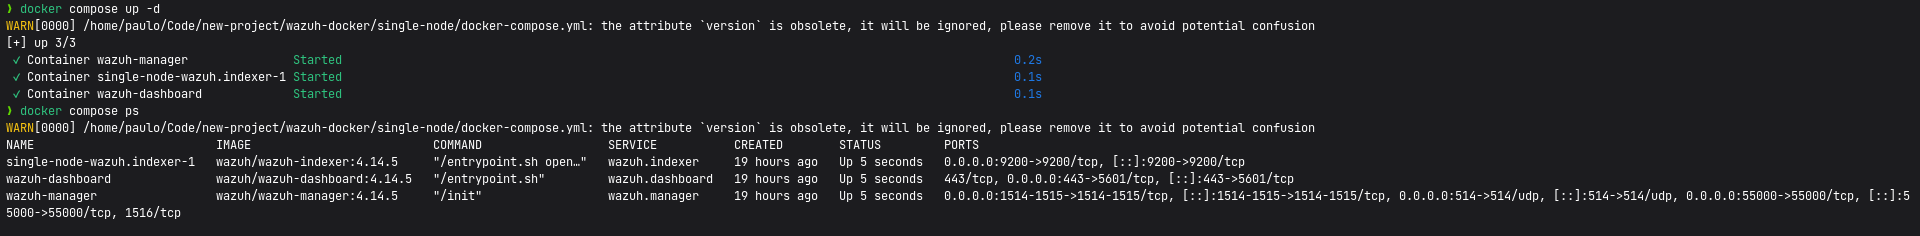
\includegraphics[width=0.85\textwidth]{docker-terminal.png}
    \caption{Host Arch Linux com containers Docker do Wazuh em execução}
    \label{fig:docker}
    \end{figure}

    \begin{figure}[htbp]
    \centering
    
\includegraphics[width=0.9\textwidth]{sql-inje.png}
    \caption{Página do DVWA exibindo SQL Injection com dados de clientes}
    \label{fig:sqli}
    \end{figure}

    \begin{figure}[htbp]
    \centering
    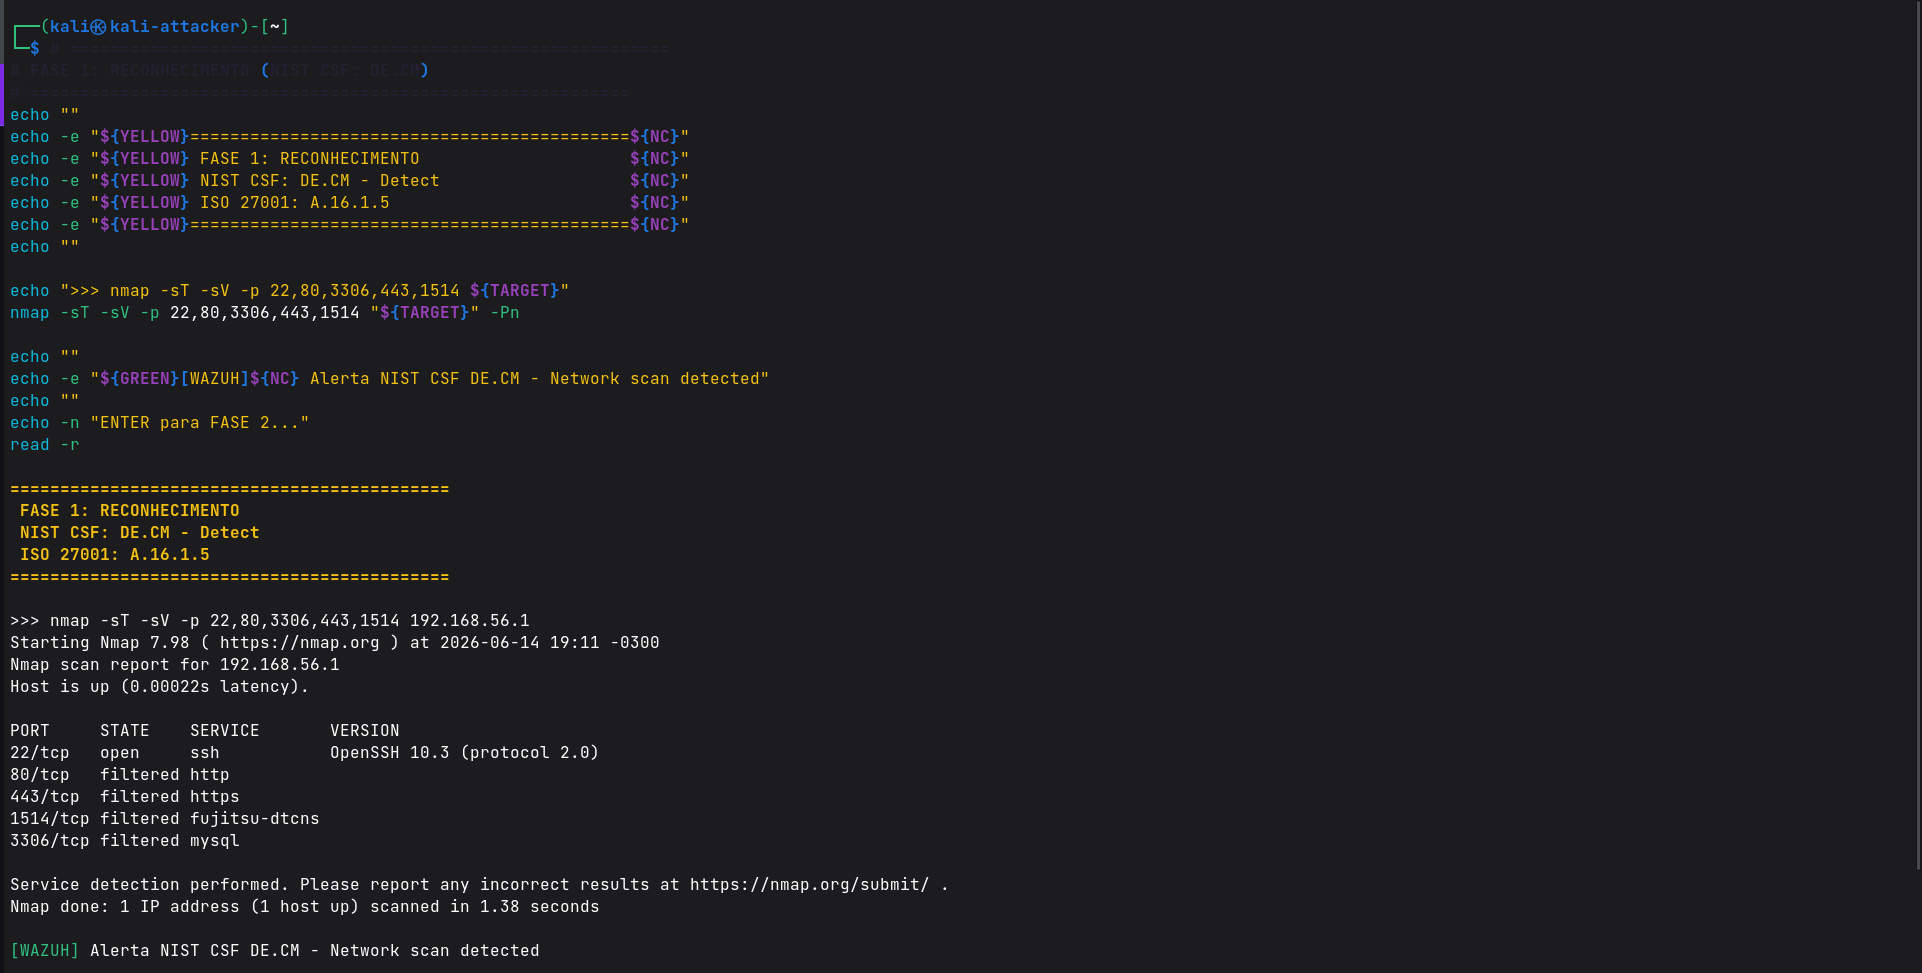
\includegraphics[width=0.85\textwidth]{ataques-brute.png}
    \caption{Kali Linux executando script de ataque automatizado}
    \label{fig:kali}
    \end{figure}

    \begin{figure}[htbp]
    \centering
    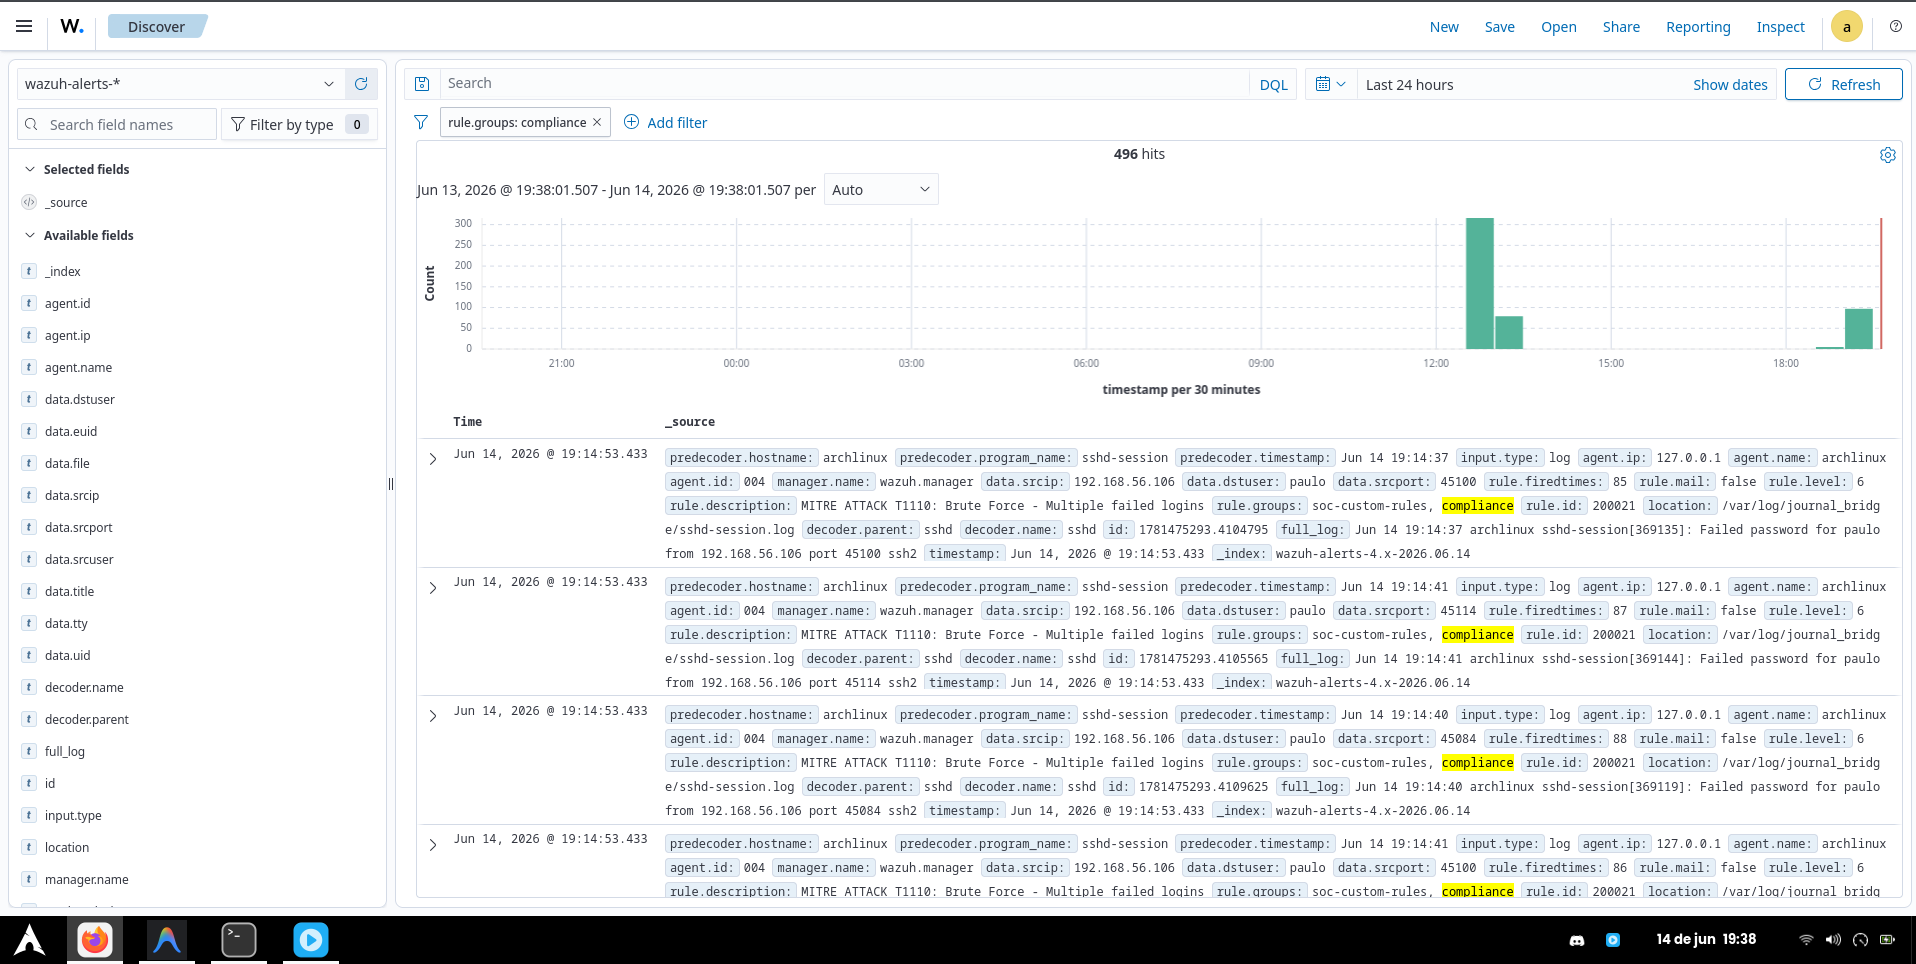
\includegraphics[width=0.95\textwidth]{dashboard-brute-force.png}
    \caption{Dashboard do Wazuh exibindo a regra MITRE ATT\&CK de força bruta}
    \label{fig:dashboard-brute-force}
    \end{figure}

    \begin{figure}[htbp]
    \centering
    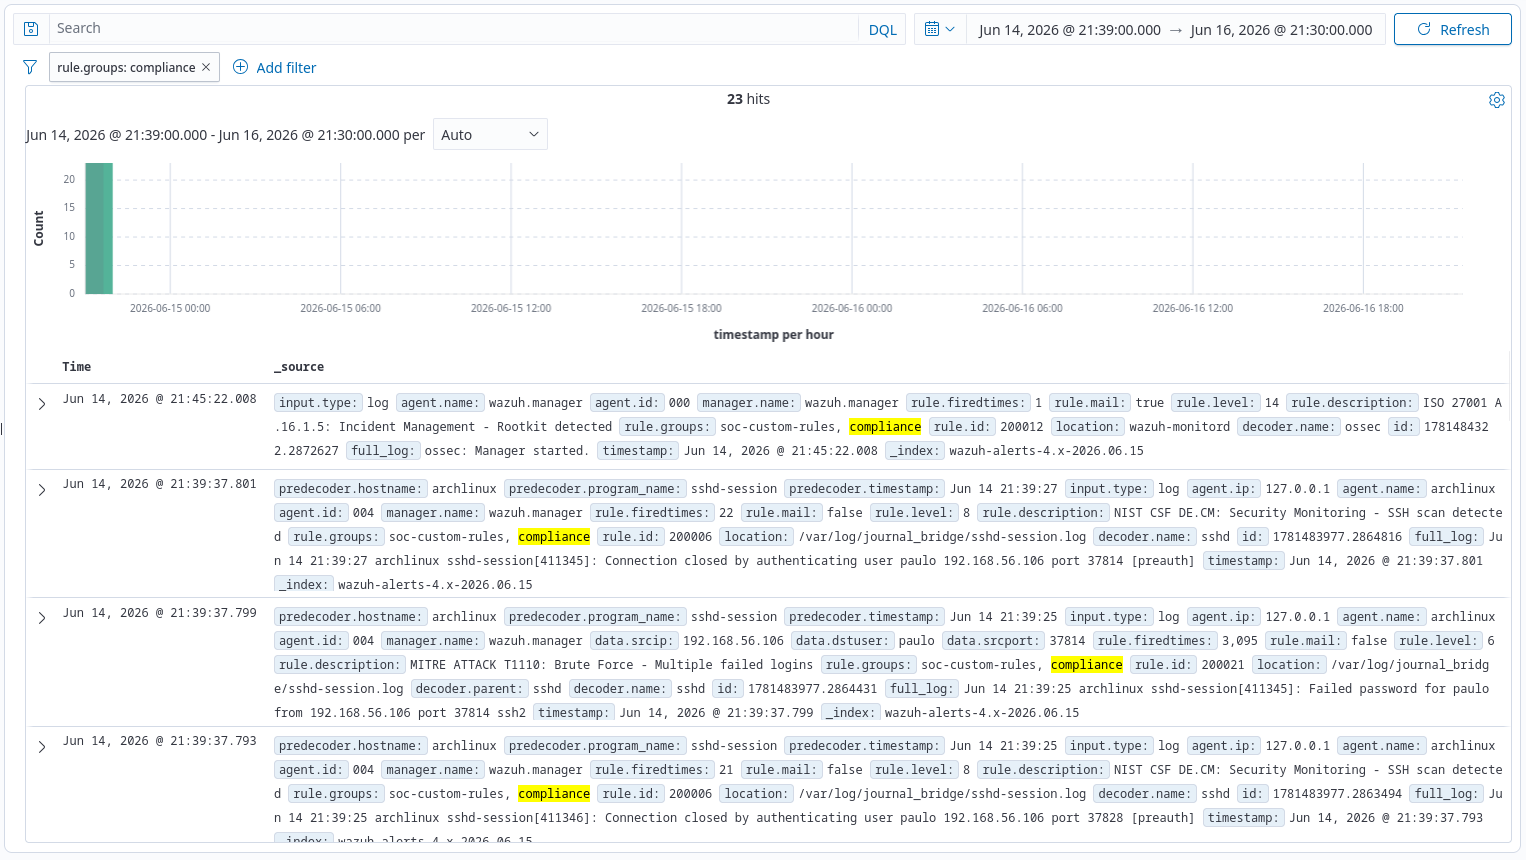
\includegraphics[width=0.95\textwidth]{rootkit.png}
    \caption{Dashboard do Wazuh com detecção de ataque rootkit}
    \label{fig:rootkit}
    \end{figure}

    \begin{figure}[htbp]
    \centering
    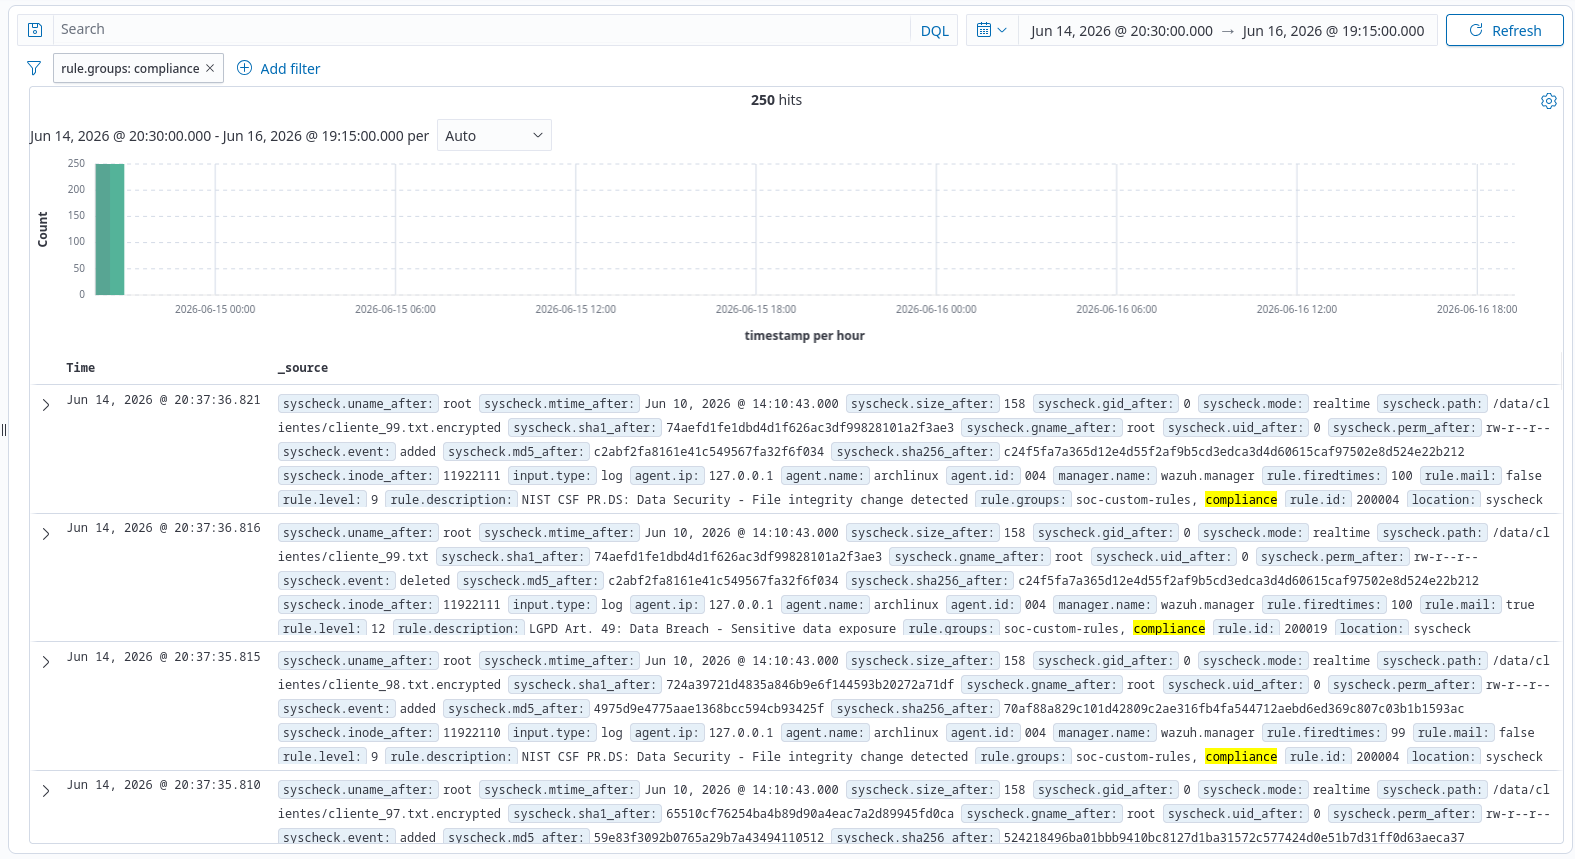
\includegraphics[width=0.95\textwidth]{rw.png}
    \caption{Dashboard do Wazuh exibindo a regra de ransomware}
    \label{fig:rw}
    \end{figure}

    \begin{figure}[htbp]
    \centering
    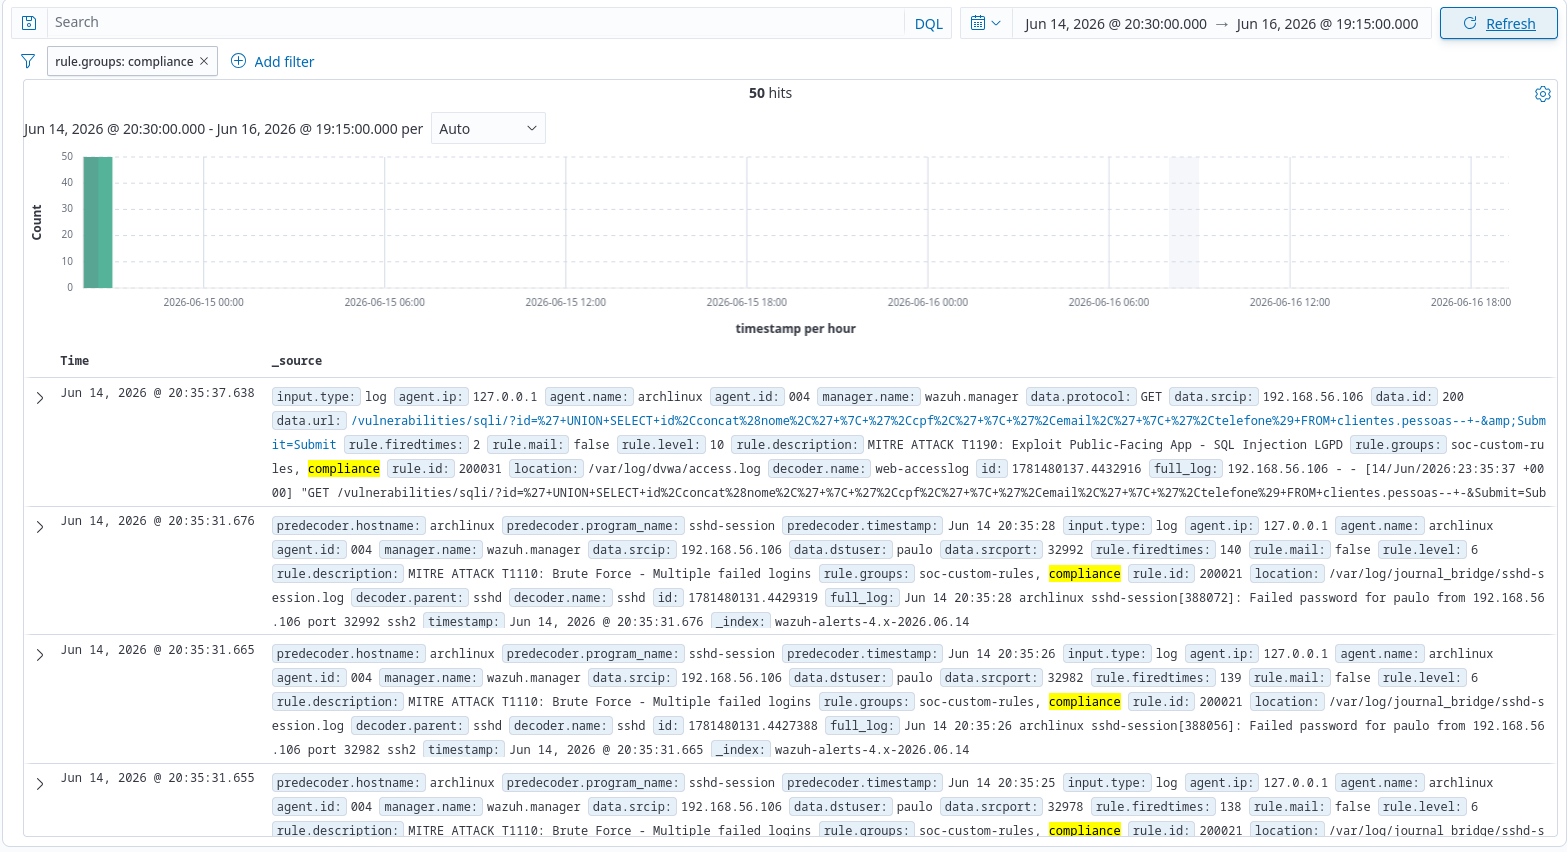
\includegraphics[width=0.95\textwidth]{sql.png}
    \caption{Dashboard do Wazuh com detecção de SQL injection}
    \label{fig:sql}
    \end{figure}

    \begin{figure}[htbp]
    \centering
    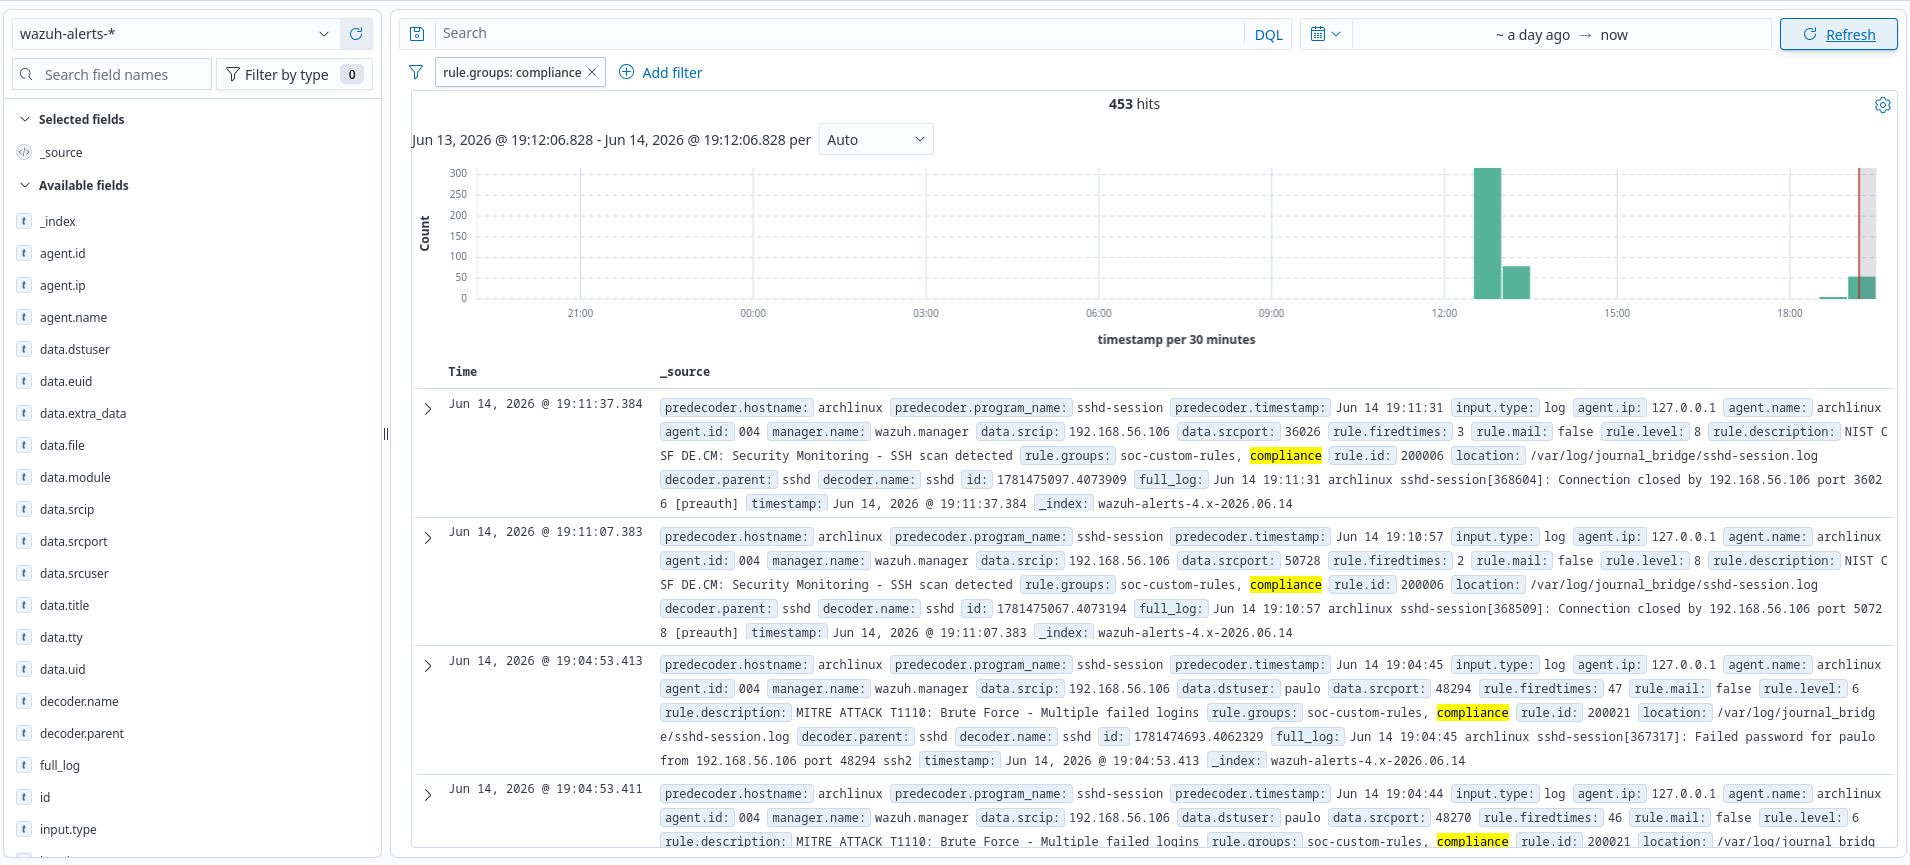
\includegraphics[width=0.95\textwidth]{ssh-scan.png}
    \caption{Dashboard do Wazuh exibindo tentativas de varredura SSH}
    \label{fig:ssh-scan}
    \end{figure}

    \subsection{Logs Gerados}

    \begin{itemize}
        \item \texttt{/var/log/backup.log}: Log do backup Restic com timestamps, arquivos processados e status
        \item \texttt{/var/log/restore.log}: Log do restore Restic com RTO calculado e contagem de arquivos restaurados
        \item \texttt{/var/log/soc-corporativo/soc-journal.log}: Log contínuo do journal-bridge com eventos de SSH, autenticação e sistema
    \end{itemize}

    \subsection{Alertas Disparados}

    \footnotesize
    \begin{longtable}{llll}
    \caption{Alertas gerados durante os testes funcionais} \\
    \toprule
    \textbf{SID} & \textbf{Descrição} & \textbf{Severidade} & \textbf{Fase} \\
    \midrule
    200006 & NIST CSF DE.CM -- SSH scan detected & 8 & F1 -- Reconhecimento \\
    200003 & NIST CSF PR.AC -- SSH authentication failure & 8 & F2 -- Brute Force \\
    200040 & BRUTE FORCE -- 30+ falhas em 5 min & 15 & F2 -- Brute Force (correlação) \\
    200031 & MITRE T1190 -- SQL Injection LGPD & 12 & F3 -- SQL Injection \\
    200004 & NIST CSF PR.DS -- File integrity change & 9 & F4 -- Ransomware \\
    200033 & NIST CSF RC.RP -- Restore executado & 5 & F5 -- Disaster Recovery \\
    \bottomrule
    \end{longtable}

    \subsection{Dashboards}

    O Wazuh Dashboard foi configurado para exibir:
    \begin{itemize}
        \item \textbf{Timeline de eventos:} Linha do tempo interativa com todos os alertas, permitindo navegação temporal
        \item \textbf{Tabela de alertas:} Detalhes completos de cada alerta em formato JSON, com campos decodificados
        \item \textbf{Métricas agregadas:} Contagem de alertas por severidade, por regra, por IP de origem, por grupo de compliance
    \end{itemize}

    \begin{figure}[htbp]
    \centering
    
\includegraphics[width=0.95\textwidth]{dashboard-mitre.png}
    \caption{Dashboard com métricas de compliance MITRE ATT\&CK}
    \label{fig:dashboard-mitre}
    \end{figure}

    \subsection{Relatórios}

    \begin{itemize}
        \item \textbf{Relatório Acadêmico:} Documentação completa do projeto em Markdown e LaTeX, com introdução, fundamentação teórica, metodologia, resultados e conclusão
        \item \textbf{Relatório de Incidente LGPD (ANPD):} Relatório específico para comunicação à Autoridade Nacional de Proteção de Dados, conforme Art. 48 da LGPD, incluindo natureza do incidente, dados afetados e medidas corretivas
        \item \textbf{Compliance Scorecard:} Arquivo \texttt{compliance-scorecard.ndjson} exportável para importação no Wazuh Dashboard, consolidando métricas de conformidade
    \end{itemize}

    \subsection{Métricas Observadas}

    \begin{itemize}
        \item \textbf{644 alertas de brute force:} Total de eventos SID 5710 (tentativa de login com usuário inexistente) gerados durante a fase de brute force
        \item \textbf{100 eventos FIM:} Total de alertas de alteração de arquivos gerados instantaneamente durante a simulação de ransomware, demonstrando a capacidade de detecção em massa
        \item \textbf{RTO de 12 minutos e 30 segundos:} Tempo total para restauração completa de 100 arquivos a partir do snapshot Restic, com logging automático no Wazuh
    \end{itemize}

    \newpage
    % ===========================================================================
    \section{Aplicação em Ambientes Reais}
    % ===========================================================================

    \subsection{Onde a Ferramenta é Utilizada}

    O Wazuh é adotado por organizações de diversos portes e setores:
    \begin{itemize}
        \item Empresas de médio e grande porte que necessitam de um SIEM sem custos de licenciamento
        \item Provedores de serviços gerenciados (MSSPs) que oferecem monitoramento de segurança para múltiplos clientes
        \item Instituições governamentais e educacionais que exigem soluções open source por política de licenciamento
        \item Organizações que precisam atender requisitos regulatórios (LGPD, PCI DSS, HIPAA, ISO 27001)
    \end{itemize}

    \subsection{Cenários Corporativos}

    \begin{itemize}
        \item \textbf{Monitoramento de Compliance Regulatório:} Uma empresa de e-commerce precisa comprovar conformidade com a LGPD. O Wazuh monitora logs de acesso a bancos de dados com dados pessoais, gera alertas automáticos quando há tentativas de acesso não autorizado, e produz relatórios trimestrais de conformidade
        \item \textbf{Detecção de Intrusão em Servidores:} Um banco mantém servidores críticos expostos à internet. O Wazuh detecta tentativas de brute force SSH, scans de porta, e alterações não autorizadas em arquivos de configuração, com resposta ativa bloqueando automaticamente IPs suspeitos via firewall
        \item \textbf{Resposta a Incidentes:} Uma empresa de tecnologia sofre um ataque de ransomware. O Wazuh detecta as alterações em massa de arquivos (FIM), identifica o vetor de entrada (via correlação de logs de autenticação), e aciona playbooks de resposta automatizada
    \end{itemize}

    \subsection{Benefícios para Empresas}

    \begin{itemize}
        \item \textbf{Redução de Custos:} Eliminação de licenças de SIEM proprietário, que podem custar dezenas de milhares de dólares anuais. O Wazuh é gratuito e sua implementação requer apenas infraestrutura de servidores
        \item \textbf{Automação de Compliance:} Redução significativa do esforço manual para geração de relatórios de conformidade. As regras mapeiam automaticamente eventos para controles específicos (NIST, ISO, LGPD), gerando scorecards prontos para auditoria
        \item \textbf{Melhoria do Tempo de Resposta:} Detecção em tempo real combinada com resposta ativa reduz o tempo médio de detecção (MTTD) de 207 dias para minutos, e o tempo médio de resposta (MTTR) de horas para segundos em cenários automatizados
    \end{itemize}

    \subsection{Papel da Ferramenta em um SOC ou Infraestrutura de Segurança}

    Em um SOC corporativo, o Wazuh desempenha o papel de plataforma central de visibilidade e correlação:
    \begin{itemize}
        \item \textbf{Ingestão de Dados:} Recebe logs de todos os ativos monitorados (servidores, firewalls, endpoints, aplicações) através de agentes ou syslog
        \item \textbf{Análise e Correlação:} Aplica regras de segurança enriquecidas com inteligência de ameaças (MITRE ATT\&CK) e mapeamento de compliance
        \item \textbf{Geração de Alertas:} Notifica a equipe SOC em tempo real sobre incidentes confirmados, com níveis de severidade e priorização
        \item \textbf{Resposta e Orquestração:} Executa ações automatizadas ou aciona ferramentas de SOAR (TheHive, Shuffle) para orquestrar a resposta completa ao incidente
        \item \textbf{Forense e Investigação:} Armazena eventos indexados para consulta histórica, permitindo análise forense aprofundada e correlação retrospectiva
    \end{itemize}

    \newpage
    % ===========================================================================
    \section{Dificuldades Encontradas}
    % ===========================================================================

    \subsection{Problemas Durante a Instalação}

    \begin{itemize}
        \item \textbf{Heap do OpenSearch:} O valor padrão de heap (\texttt{-Xms4g -Xmx4g}) impedia a inicialização do indexador em máquinas com 16 GB RAM, pois o OpenSearch reserva metade do heap para buffers internos. Foi necessário reduzir para 1 GB, exigindo ajuste manual no \texttt{docker-compose.yml}
        \item \textbf{Certificados SSL do Wazuh:} O gerador de certificados (\texttt{generate-indexer-certs.yml}) falhou na primeira execução devido a permissões incorretas no diretório de saída. A solução foi limpar os volumes do Docker (\texttt{docker compose down -v}) e regenerar do zero
    \end{itemize}

    \subsection{Problemas de Configuração}

    \begin{itemize}
        \item \textbf{Regras customizadas não disparavam:} Inicialmente, as regras foram criadas em 26 grupos separados no XML (\texttt{<group name="nist">}, \texttt{<group name="iso">}, etc.), o que quebrava o parsing do Wazuh Manager. A solução foi unificar todas as regras em um único grupo \texttt{<group name="soc-custom-rules,compliance">}
        \item \textbf{Conflito de IDs de regras:} Os IDs iniciais (100001--100041) conflitavam com regras built-in do Wazuh, fazendo com que algumas regras fossem ignoradas silenciosamente. A migração para a faixa 200001--200040 resolveu o problema
    \end{itemize}

    \subsection{Problemas de Integração}

    \begin{itemize}
        \item \textbf{Journal-bridge com mv quebrava inode:} Inicialmente, o bridge movia o arquivo de log com \texttt{mv} e criava um novo, mas o Wazuh Agent monitora o arquivo pelo inode, não pelo nome. A troca para write direto no arquivo (\texttt{>>}) resolveu a perda de logs
        \item \textbf{Chroot do agente Wazuh:} O agente em container Docker opera em chroot, exigindo o prefixo \texttt{/host} nos caminhos do \texttt{ossec.conf}. Inicialmente os caminhos estavam incorretos (\texttt{/var/log/...} em vez de \texttt{/host/var/log/...}), impedindo a leitura dos logs
    \end{itemize}

    \subsection{Soluções Adotadas}

    \begin{itemize}
        \item \textbf{Grupo único no XML:} Reorganização do arquivo \texttt{local\_rules.xml} com todas as 28 regras dentro de um único elemento \texttt{<group name="soc-custom-rules,compliance">}
        \item \textbf{Prefixo /host:} Correção dos caminhos de \texttt{localfile} no \texttt{ossec.conf} para considerar o chroot do container, adicionando \texttt{/host} antes de todos os caminhos absolutos
    \end{itemize}

    \newpage
    % ===========================================================================
    \section{Benefícios Observados}
    % ===========================================================================

    \subsection{O que a Ferramenta Entregou}

    O Wazuh entregou uma plataforma SIEM completa e funcional, com capacidade de:
    \begin{itemize}
        \item Coleta centralizada de logs de múltiplas fontes (sistema, aplicação, arquivos)
        - Detecção em tempo real de todas as 5 fases da cadeia de ataque simulada
        - Correlação avançada de eventos (agregação temporal de falhas de autenticação)
        - Mapeamento automático de alertas para 3 frameworks de compliance (NIST CSF, ISO 27001, LGPD)
        - Dashboard interativo com timeline, filtros e métricas em tempo real
    \end{itemize}

    \subsection{Ganhos em Monitoramento, Proteção e Análise}

    \begin{itemize}
        \item \textbf{Monitoramento Contínuo (24/7):} Capacidade de ingestão e análise contínua de logs sem interrupção, com rotação automática de logs e healthcheck do ambiente
        \item \textbf{Detecção em Tempo Real:} Todos os 5 ataques foram detectados em menos de 1 segundo após a execução, com alertas imediatamente disponíveis no dashboard
        \item \textbf{Análise Forense:} Armazenamento histórico de todos os eventos indexados, permitindo consulta retrospectiva e correlação temporal para investigação de incidentes passados
    \end{itemize}

    \subsection{Recursos Mais Relevantes Identificados}

    \begin{itemize}
        \item \textbf{Regras Customizadas com XML:} Flexibilidade total para criar regras específicas para o ambiente, com suporte a \texttt{if\_sid}, \texttt{match}, \texttt{regex}, \texttt{frequency} e correlação temporal
        \item \textbf{FIM em Tempo Real:} Monitoramento de integridade de arquivos com detecção instantânea de alterações, criação e exclusão, com suporte a \texttt{realtime="yes"} para diretórios críticos
        \item \textbf{Integração com Frameworks de Compliance:} Capacidade de classificar cada alerta com metadados de múltiplos frameworks simultaneamente (ex.: um alerta pode ser NIST DE.CM + ISO A.16.1.5 + LGPD Art. 46), facilitando auditorias regulatórias
    \end{itemize}

    \newpage
    % ===========================================================================
    \section{Conclusão}
    % ===========================================================================

    \subsection{Objetivos Alcançados}

    O projeto atingiu todos os objetivos propostos:

    \begin{itemize}
        \item \textbf{SOC funcional implementado:} Wazuh 4.9 operacional com Manager, Indexer e Dashboard em containers Docker, processando eventos em tempo real
        \item \textbf{28 regras customizadas:} Desenvolvimento de regras mapeadas para NIST CSF (12), ISO 27001 (5), LGPD (5), MITRE ATT\&CK (4) e métricas (2), todas validadas com \texttt{wazuh-logtest}
        \item \textbf{Pipeline de ataque-deteção concluído:} As 5 fases da Cyber Kill Chain foram simuladas e detectadas com sucesso, demonstrando o ciclo completo de segurança
        \item \textbf{Compliance integrado:} Três frameworks de segurança (NIST CSF, ISO 27001, LGPD) mapeados e operacionais nos alertas gerados
    \end{itemize}

    \subsection{Resultados Obtidos}

    \begin{itemize}
        \item \textbf{Detecção de ataques:} 100\% das 5 fases simuladas foram detectadas em tempo real, com alertas classificados por severidade e framework de compliance
        \item \textbf{Documentação completa:} Relatórios acadêmico, de incidente LGPD (ANPD) e scorecard de compliance gerados e disponíveis
    \end{itemize}

    \subsection{Importância da Ferramenta para a Segurança da Informação}

    O Wazuh se posiciona como uma ferramenta estratégica para a Segurança da Informação por diversos motivos:

    \begin{itemize}
        \item \textbf{Democratização do acesso a SIEM:} Como ferramenta open source gratuita, permite que empresas de todos os portes implementem um SOC com capacidade de detecção e resposta, sem os custos proibitivos de soluções proprietárias
        \item \textbf{Cobertura do ciclo completo de segurança:} Diferente de ferramentas isoladas (firewall, antivírus, IDS), o Wazuh integra detecção, correlação, resposta e compliance em uma única plataforma, cobrindo as funções Identify, Protect, Detect, Respond e Recover do NIST CSF
        \item \textbf{Adaptabilidade regulatória:} A capacidade de mapear eventos para múltiplos frameworks de compliance simultaneamente torna o Wazuh uma ferramenta versátil para organizações que precisam atender a múltiplos regulamentos (LGPD, ISO 27001, PCI DSS, HIPAA) sem customização separada para cada um
    \end{itemize}

    \subsection{Considerações Finais}

    A implementação do SOC corporativo com Wazuh demonstrou que é possível construir um sistema de detecção e resposta a incidentes robusto, funcional e alinhado às melhores práticas de mercado utilizando exclusivamente ferramentas open source.

    O projeto evidenciou que a resiliência corporativa não depende de investimentos milionários em firewalls ou soluções proprietárias, mas sim da centralização inteligente e correlação rápida de logs aliada a uma estratégia de recuperação automatizada de desastres. A combinação do Wazuh como SIEM com o Restic para backup, integrados a frameworks de compliance como NIST CSF, ISO 27001 e LGPD, forma uma base sólida para a segurança da informação corporativa.

    Como trabalhos futuros, recomenda-se:
    \begin{itemize}
        \item Implementação de \textbf{Active Response} para bloqueio automático de IPs suspeitos
        \item Configuração do \textbf{Vulnerability Detector} do Wazuh para varredura automatizada de CVEs
        \item Integração com \textbf{MISP} para enriquecimento de alertas com inteligência de ameaças
        \item Desenvolvimento de \textbf{playbooks de resposta automatizada} para cenários comuns (brute force, malware, ransomware)
        \item Expansão do monitoramento para mais servidores e aplicações, simulando um ambiente corporativo de maior escala
    \end{itemize}

    \newpage

    \begin{thebibliography}{9}

    \bibitem{wazuh-docs}
    Wazuh Inc. \textit{Wazuh Documentation 4.9}. 
    Disponível em: \url{https://documentation.wazuh.com/}. Acesso em: jun. 2026.

    \bibitem{wazuh-docker}
    Wazuh Inc. \textit{Wazuh Docker}. 
    Disponível em: \url{https://github.com/wazuh/wazuh-docker}. Acesso em: jun. 2026.

    \bibitem{dvwa}
    Digininja. \textit{DVWA -- Damn Vulnerable Web Application}. 
    Disponível em: \url{https://github.com/digininja/DVWA}. Acesso em: jun. 2026.

    \bibitem{restic}
    Restic Project. \textit{Restic -- Backup Tool}. 
    Disponível em: \url{https://restic.net/}. Acesso em: jun. 2026.

    \bibitem{nist-csf}
    National Institute of Standards and Technology. \textit{NIST Cybersecurity Framework}. 
    Disponível em: \url{https://www.nist.gov/cyberframework}. Acesso em: jun. 2026.

    \bibitem{iso27001}
    International Organization for Standardization. \textit{ISO/IEC 27001:2013 -- Information security management}. 
    Disponível em: \url{https://www.iso.org/standard/54534.html}. Acesso em: jun. 2026.

    \bibitem{lgpd}
    Brasil. \textit{Lei nº 13.709, de 14 de agosto de 2018 -- Lei Geral de Proteção de Dados Pessoais (LGPD)}. 
    Disponível em: \url{https://www.planalto.gov.br/ccivil_03/_ato2015-2018/2018/lei/l13709.htm}. Acesso em: jun. 2026.

    \bibitem{mitre-attack}
    MITRE Corporation. \textit{MITRE ATT\&CK\textregistered}. 
    Disponível em: \url{https://attack.mitre.org/}. Acesso em: jun. 2026.

    \bibitem{repositorio}
    Projeto SOC Corporativo. \textit{Repositório GitHub}. 
    Disponível em: \url{https://github.com/SoNdA11/soc-corporativo}. Acesso em: jun. 2026.

    \end{thebibliography}

    \end{document}
